% !TEX root = 00_main.tex
\chapter{提案手法}\label{chap:method}
本章では，提案手法について述べる．
以下に，論文でよく使う記法の例を示す（不要になったら削除してよい）．

\section{図の挿入例}
図は\verb|graphics/|ディレクトリに PDF 形式で置き，\figref{sample}のように参照する．

\begin{figure}[htb]
  \centering
  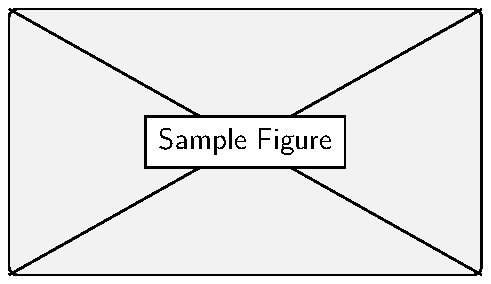
\includegraphics[width=0.6\textwidth]{graphics/sample.pdf}
  \caption{サンプル図}
  \label{fig:sample}
\end{figure}

\section{表の挿入例}
表は\tabref{sample}のように参照する．
表のキャプションは表の上に，図のキャプションは図の下に置くのが一般的である．

\begin{table}[htb]
  \centering
  \caption{サンプル表}
  \label{tab:sample}
  \begin{tabular}{|l|c|c|} \hline
    手法     & 精度 [\%] & 処理時間 [s] \\ \hline \hline
    従来手法 & 80.0      & 1.2          \\ \hline
    提案手法 & 90.0      & 0.8          \\ \hline
  \end{tabular}
\end{table}

\section{数式の例}
番号付きの数式は\equref{sample}のように参照する．
\begin{equation}
  E = \frac{1}{N} \sum_{i=1}^{N} (y_i - \hat{y}_i)^2
  \label{eq:sample}
\end{equation}
文中の数式は $x^2 + y^2 = r^2$ のように書く．

\section{箇条書きの例}
\begin{itemize}
  \item 項目1
  \item 項目2
\end{itemize}

\begin{enumerate}
  \item 手順1
  \item 手順2
\end{enumerate}

\section{コメントアウト}
% 1行だけなら % を使う．
\begin{comment}
  複数行をまとめて PDF に出力しないようにするには
  comment 環境を使う．
\end{comment}
メモや下書きは\verb|%|や\verb|comment|環境で残しておくとよい．
